\documentclass[border=0pt]{standalone}
\usepackage{fontspec}
\setmainfont{Liberation Serif}
\usepackage{unicode-math}
\setmathfont{latinmodern-math.otf}
\usepackage{tkz-euclide}
\usetikzlibrary{arrows.meta,calc,intersections,decorations.markings,angles,quotes}

% tkz-euclide assumes centimetre coordinates. Fonts and strokes use print sizes.
\tikzset{
  every picture/.style={x=1cm,y=1cm,line width=.55pt,line cap=round,line join=round,font=\fontsize{11}{13}\selectfont},
  every node/.style={inner sep=2pt},
  construction/.style={densely dashed,line width=.4pt},
  dimension/.style={<->,>=Stealth,line width=.4pt},
  vector/.style={postaction=decorate,decoration={markings,mark=at position .55 with {\arrow{Stealth[length=4pt,width=3pt]}}}},
  note/.style={font=\fontsize{9}{11}\selectfont\itshape,draw=black!65,line width=.35pt,inner sep=3pt,align=center},
  point/.style={circle,fill=black,inner sep=0pt,minimum size=1.8pt},
  axis/.style={-{Stealth[length=4pt,width=3pt]},line width=.45pt}
}
\newcommand{\NotToScale}[1]{\node[note] at #1 {Diagram is\\NOT to scale};}
% Fix the output canvas so Typst does not resize typography to fit label extents.
\newcommand{\ExamBounds}[2]{\pgfresetboundingbox\path[use as bounding box] (0,0) rectangle (#1mm,#2mm);}

\begin{document}
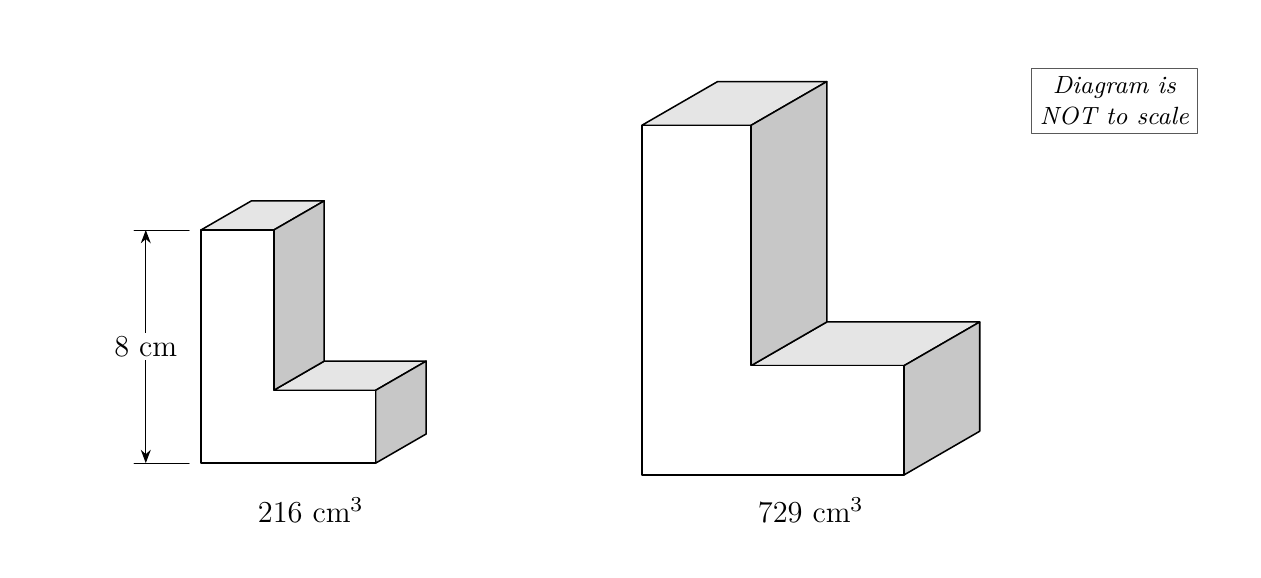
\begin{tikzpicture}
  % One L-shaped duct drawn twice; the larger copy is 1.5 times the smaller
  % (volume ratio 216 : 729 = 1 : 3.375 = 1 : 1.5^3). Page coordinates in cm; duct model at 3.7 mm per cm.
  \newcommand{\duct}[2]{%
    \begin{scope}[shift={#1},x={(#2*3.7mm,0mm)},y={(#2*1.602mm,#2*.925mm)},z={(0mm,#2*3.7mm)}]
      \filldraw[fill=black!10] (0,0,8) -- (2.5,0,8) -- (2.5,4,8) -- (0,4,8) -- cycle;
      \filldraw[fill=black!10] (2.5,0,2.5) -- (6,0,2.5) -- (6,4,2.5) -- (2.5,4,2.5) -- cycle;
      \filldraw[fill=black!22] (2.5,0,2.5) -- (2.5,4,2.5) -- (2.5,4,8) -- (2.5,0,8) -- cycle;
      \filldraw[fill=black!22] (6,0,0) -- (6,4,0) -- (6,4,2.5) -- (6,0,2.5) -- cycle;
      \filldraw[fill=white] (0,0,0) -- (6,0,0) -- (6,0,2.5) -- (2.5,0,2.5) -- (2.5,0,8) -- (0,0,8) -- cycle;
    \end{scope}}
  \duct{(2.2,1.1)}{1}
  \duct{(7.8,.95)}{1.5}
  \draw[line width=.3pt] (2.05,1.1) -- (1.35,1.1) (2.05,4.06) -- (1.35,4.06);
  \draw[dimension] (1.5,1.1) -- node[fill=white,inner sep=1pt] {8 cm} (1.5,4.06);
  \node at (3.6,.5) {216 cm$^3$};
  \node at (9.95,.5) {729 cm$^3$};
  \NotToScale{(13.8,5.7)}
  \ExamBounds{153}{66.3}
\end{tikzpicture}
\end{document}
